\documentclass{article}
\usepackage{lipsum}
\usepackage{amsmath}
\usepackage{hyperref}
\usepackage{xcolor}
\usepackage{amsfonts}
\usepackage{graphicx}

\usepackage{enumitem}
\setlist[enumerate]{itemsep=-1mm}


\topmargin=-0.65in    % Make letterhead sftart about 1 inch from top of page
\textheight=9.10in    % text height can be bigger for a longer letter
\oddsidemargin=-0.1in % leftmargin is 1 inch
\textwidth=6.7in   % textwidth of 6.5in leaves 1 inch for right margin

% some shortcuts
\newcommand{\ea}{\textit{et al. }} 
\newcommand{\ttt}[1]{\texttt{#1}}
\newcommand{\eg}{\textit{e.g. }} 
\newcommand{\ie}{\textit{i.e. }} 
\newcommand{\la}{\langle}
\newcommand{\ra}{\rangle}
\newcommand{\cg}{\color{gray}}
\newcommand{\fs}{\footnotesize}
\setlength{\parindent}{0mm}


%%%%%%%%%%%%%%%%%%%%%%%%%%%%%%%%%%%%%%%%%%%%%%%%%%%%%%%%%%%%%%%%%%%%%%%%
%%%%%%%%%%%%%%%%%%%%%%%%%%%%%%%%%%%%%%%%%%%%%%%%%%%%%%%%%%%%%%%%%%%%%%%%
%%%%%%%%%%%%%%%%%%%%%%%%%%%%%%%%%%%%%%%%%%%%%%%%%%%%%%%%%%%%%%%%%%%%%%%%
%%%%%%%%%%%%%%%%%%%%%%%%%%%%%%%%%%%%%%%%%%%%%%%%%%%%%%%%%%%%%%%%%%%%%%%%
\begin{document}


%%%%%%%%%%%%%%%%%%%%%%%%%%%%%%%%%%%%%%%%%%%%%%%%%%%%%%%%%%%%%%%%%%%%%%%%
%%%%%%%%%%%%%%%%%%%%%%%%%%%%%%% OUTLINE %%%%%%%%%%%%%%%%%%%%%%%%%%%%%%%%
%%%%%%%%%%%%%%%%%%%%%%%%%%%%%%%%%%%%%%%%%%%%%%%%%%%%%%%%%%%%%%%%%%%%%%%%
\title{\bf Filter Design Cheatsheet}
\maketitle

\section{FIR Filter Design}
This cheatsheet is compiled from book Digital Signal Processing with MATLAB by Ingle \& Proakis. Page references are given as \#PageNo

\paragraph{Problem Statement}
Design a lowpass filter that has a passband $[0,\omega_p]$ with tolerance $\delta_1$ (or $R_p$ in dB) and a stopband $[\omega_s, \pi]$ with tolerance $\delta_2$ (or $A_s$ in dB) \---- see Figure \ref{fig:design}b,c.

In FIR we focus on linear-phase filters:
\begin{equation}
H(e^{j\omega})=H_r(\omega)e^{j(\beta-\alpha\omega)}
\end{equation}

where $\alpha$ is \textit{constant group delay} and $H_r$ is the amplitude. The impulse response of linear-phase filters is symmetric or antisymmetric about $alpha$, therefore $\alpha=\frac{M-1}{2}$ and $h(n)=h(M-1-n)$ where $M$ is the filter length. A central goal in FIR filter design is to keep $M$ minimal. Based on whether the filter is symmetric or anti-symmetric, and whether $M$ is odd or even, there are four types of filters well-accepted in the literature. Each of these filters has a different usage.:

\begin{table}[h]
\centering
\begin{tabular}{|l|l|l|l|l|} \hline
 & M & symm/anti-symm  & $\beta$ & usage \\ \hline
\textbf{Type I} & odd & symm & 0 & lowpass, highpass, bandstop \\
\textbf{Type II} & even & symm & 0 & lowpass only (not highpass or bandstop (see \#233)) \\
\textbf{Type III} & odd & anti-symm & $\pi/2$ & dig. Hilbert transformers and differentiators (for derivative)\\
\textbf{Type IV} & even & anti-symm & $\pi/2$ & dig. Hilbert transformers and differentiators (for derivative)\\ \hline
\end{tabular}
\caption{Filter types}
\label{tab:types}
\end{table}

\subsection{Design approaches}
\begin{enumerate}
\item Windowing an ideal LP filter
\item Designing directly in Frequency Domain
\item Optimal equiripple design
\end{enumerate}

The first two are intuitive but not optimal. The third has a more sophisticated theory but is optimal. Optimality here means minimal $M$ for given design specs (\ie desired $\omega_p, \omega_s, R_p, A_s$ values).

\subsubsection{Windowing an ideal lowpass filter}
An ideal lowpass (LP) filter (see Fig. \ref{fig:design}a) must be infinite. To make it FIR we must truncate the ideal filter, which will introduce ripples around cutoff frequency (see Fig. \ref{fig:design}b) due to Gibbs phenomenon (see \#245 onwards). The truncation is done by windowing, \ie multiplication (or conv in freq domain) with a windowing function. The goal  is to find the windowing function that meets the design specs with minimal $M$. The simplest and worse-performing windowing fn is boxcar. More sophisticate ones are triangular, Hanning, Hamming and Blackman. Hamming is typically used. See \#251 for comparison among windows.

\subsubsection{Designing directly in Frequency Domain}
We manually design a sequence in frequency domain such as $H(k) = \{1,1,1,1,0,0,0,0,0,0,0\}$ (number of 1's is proportional to $\omega_c$). This would be the freq response of the ideal filter. To minimize ripples, we manually introduce a slope such as $H(k) = \{1,1,1,T_1,T_2,0,0,0,0\}$. We decide the number of $T_i$ values, then the goal is to find the optimal $T_i$ values. See \#264 onwards.

\subsubsection{Optimal Equiriple Design}
It turns out that the optimal design is reached by distributing the error around ripples uniformly (in contrary to having an increasing error nearer the band edges). This can be performed with by solving what is called a \textit{minimax problem} (see \#278 onwards). This requires a polynomial approximation which is performed via the Parks-McClellan algorithm (\#284). 

All these can be done very simply in MATLAB through the \ttt{remez} function. The overall design is as follows:
\begin{enumerate}
\item Decide specs: $\omega_p, \omega_s, R_p, A_s$
\item Guess an initial filter length $\hat{M}$ (see code and 7.48 in \#284)
\item Run \ttt{remez}
\item check $A_s$, if OK stop, if not, increase $\hat{M}$ and repeat until desired $A_s$ reached. Bear in mind that the restrictions on $M$ based on the filter usage (see Table \ref{tab:types}) still apply and therefore $M$ should be incremented carefully (\ie maintain an either odd or even value).
\end{enumerate}


Exemplar piece of code to create bandpass filter: 
{
\footnotesize
\begin{verbatim}
% Filter specifications
Rp = 0.5; As = 50;
ws1 = 0.2*pi; wp1 = 0.3*pi; wp2 = 0.7*pi; ws2 = 0.8*pi;

% deltas are defined through simple equations, see #226
delta1 = (10^(Rp/20)-1)*(10^(Rp/20)+1);
delta2 = (1+delta1)*(10^(-As/20));

deltaH = max(delta1, delta2); deltaL = min(delta1, delta2);
delta_f = min((ws2-wp2)/(2*pi), (wp1-ws1)/(2*pi)); see #284

% Compute initial M, see #284
M = ceil((-20*log10(sqrt(delta1*delta2))-13)/(14.6*delta_f)+1);
if mod(M,2) == 0; M = M+1; end

f = [0 ws1/pi wp1/pi wp2/pi ws2/pi  1]; % key frequency values (normalized to range [0,1])
m = [0 0 1 1 0 0]; % desired magnitude values at above frequencies
weights = [1 delta2/delta1 1]; % weight parameter needed by equiripple design theory, see #280

h = remez(M-1,f,m,weights); % create the filter
[H,w] = freqz(h,1,1000,'whole'); % Filter in frequency domain

% Plot
H = (H(1:1:501))'; w = (w(1:1:501))';
mag = abs(H);
db = 20*log10((mag+eps)/max(mag));

% Now check if we met constraints
delta_w = 2*pi/1000; ws1i = floor(ws1/delta_w)+1;
Asd = -max(db(1:1:ws1i))

% Not enough min attenuation, we need to increment a bit more
M = M+2;
h = remez(M-1,f,m,weights); % create the filter
[H,w] = freqz(h,1,1000,'whole'); % Filter in frequency domain

% Plot
H = (H(1:1:501))'; w = (w(1:1:501))'; mag = abs(H);
db = 20*log10((mag+eps)/max(mag));

subplot(2,1,1); plot(w/500/(2*pi),mag) ylim([0 1.3]);
subplot(2,1,2); plot(w/500/(2*pi),db); ylim([-100 2]);
\end{verbatim}
}







\clearpage
\section{IIR Filter Design}
The idea is to first design an analogue filter, then convert it to a digital one. There are 3 types of prototypical analogue filters: i) Butterworth, ii) Chebyshev (Chebysev I and II) and iii) Elliptical \---- see Fig. \ref{fig:IIR}. Butterworth has no ripples and its phase response is the closest to linear but produces the widest transition band for a filter order $N$. Elliptical has ripples on both passband and stopband and the most nonlinear phase, but produces the narrowest transition band for same $N$. Chebyshev is somewhere between the two in terms of transition bandwidth and phase linearity, and has ripples only on passband. 

\subsection{Converting to Digital} The analogue design is carried out in $s$ domain, we will convert to $z$ domain (A/D conversion). Different conversion designs retain different characteristics of the filter. One is \textit{impulse invariant design} which retains the shape of the analog impulse response after conversion to digital (\#327) and also retains stability, but possibly creates aliasing frequency response. The standard A/D conversion scheme is bilinear transformation which is not only stable but also has no aliasing (due to one-to-one mapping from $s$- to $z$-domain) and can also be applied to any type of filter (\#344).

\subsection{Filter Design in MATLAB with Bilinear Transform}
See \#339 for non-MATLAB summary. Here we consider using MATLAB functions.

We first decide the digital filter specifications $\omega_p$,$\omega_s$, $R_p$, $A_s$. % $A_s$ is needed only by elliptic filters (due to ripples in stopband) and $R_p$ is needed only by elliptic and Chebyshev filters. 
Then we use the following functions to compute the right $N$ and $\omega_n$ values:
\begin{verbatim}
[N,wn] = buttord(wp/pi, ws/pi, Rp, As); % for butterworth filter
[N,wn] = cheb1ord(wp/pi, ws/pi, Rp, As); % for chebyshev I
[N,wn] = cheb2ord(wp/pi, ws/pi, Rp, As); % for chebyshev II
[N,wn] = ellipord(wp/pi, ws/pi, Rp, As); % for elliptic
\end{verbatim}

Then we feed these parameters to the filter implementation functions:
\begin{verbatim}
[b,a] = butter(N, wn,'filterType') % filterType is 'high', 'stop' etc. see doc.
[b,a] = cheby1(N, Rp, wn, 'filterType')
[b,a] = cheby2(N, Rp, wn, 'filterType')
[b,a] = ellip(N, Rp, As, wn, 'filterType')
\end{verbatim}

The output \ttt{b,a} are the nominator and denominator of the filter function in $z$ domain. We perform filtering via the \ttt{filter(b,a,x)} function.


\begin{figure}
\centering
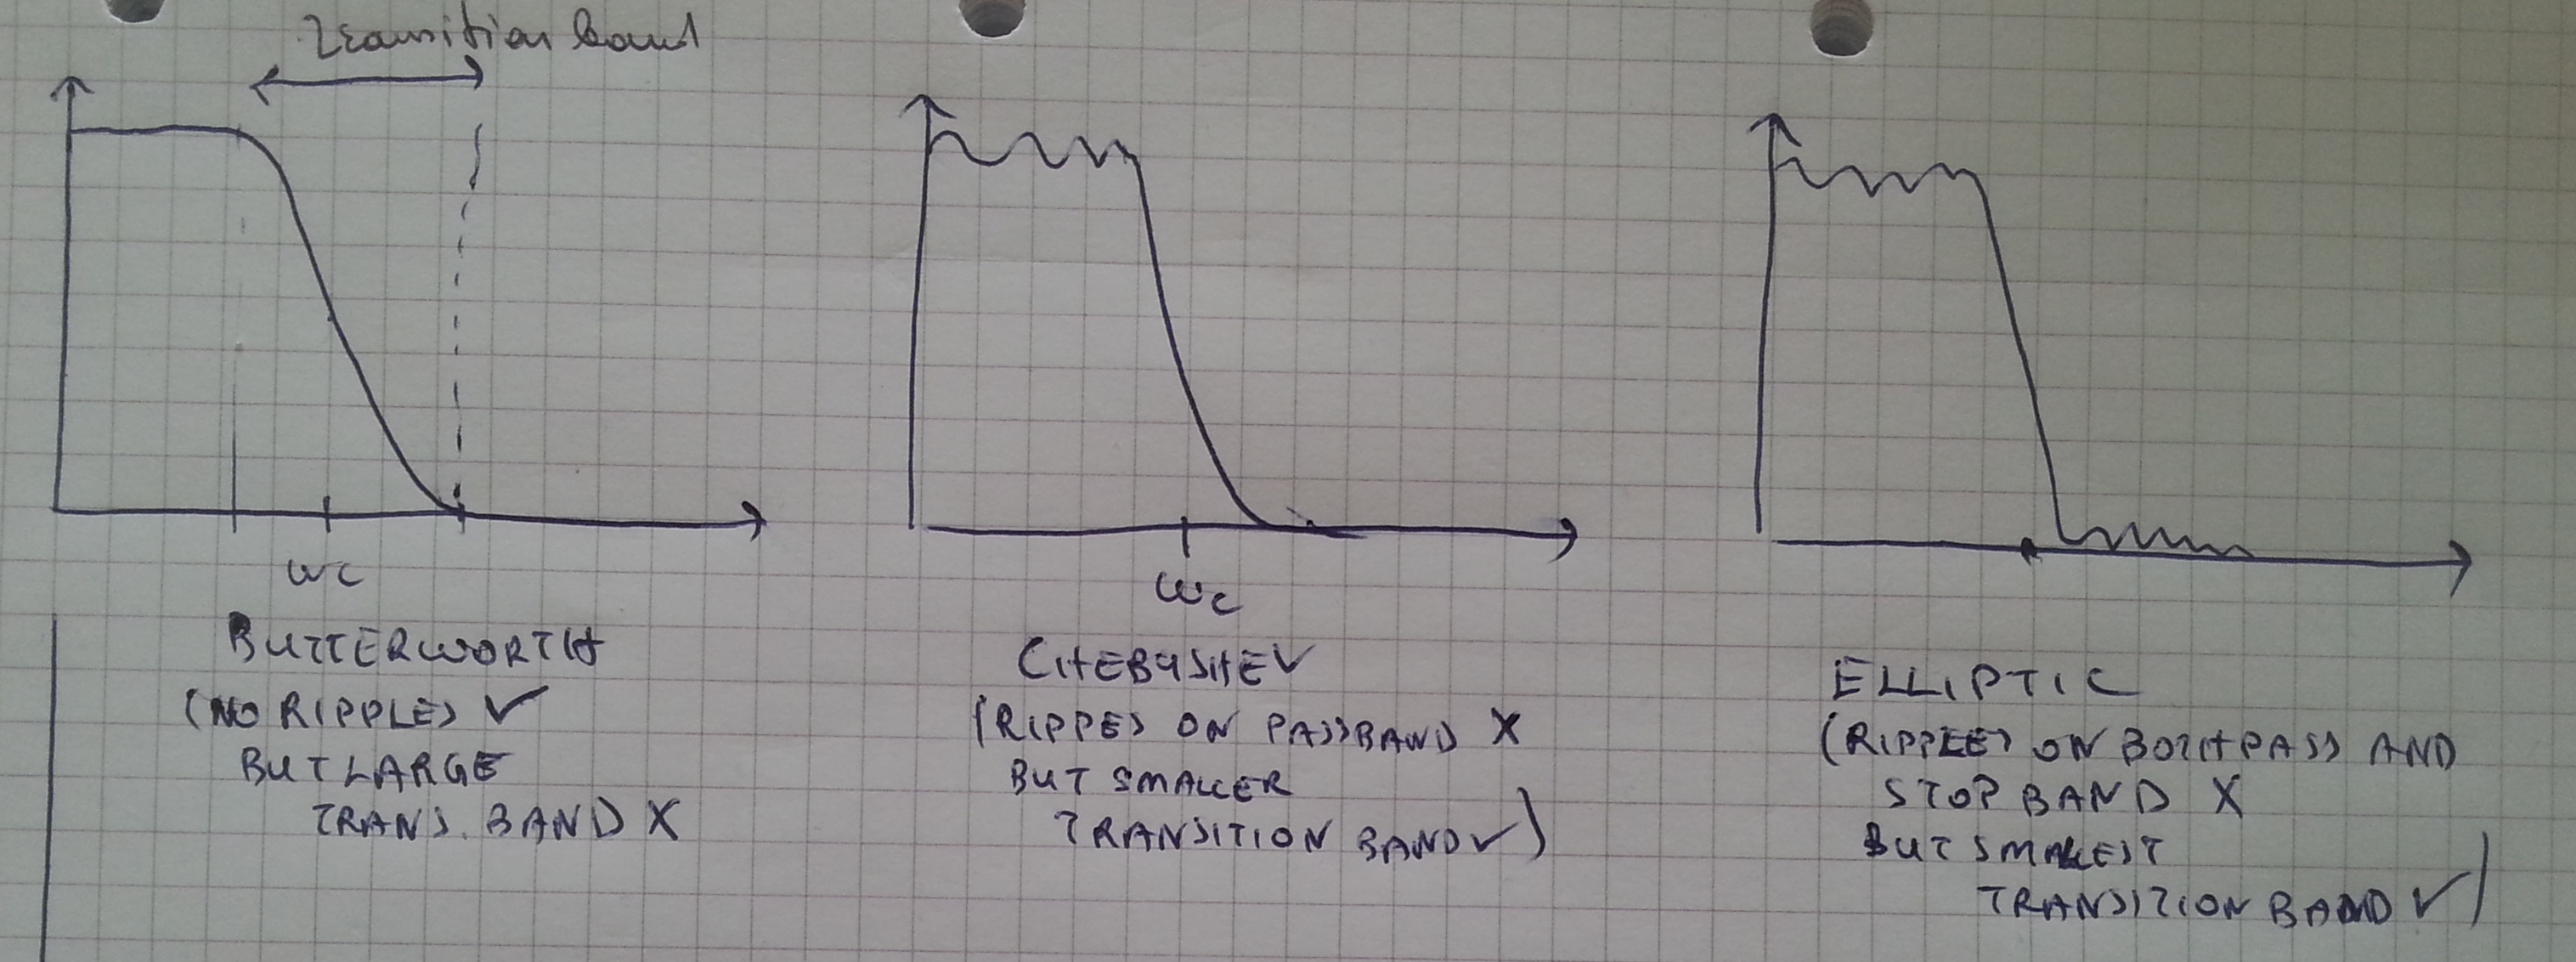
\includegraphics[scale=0.13]{fig/iir_design.jpg}
\label{fig:iir}
\caption{IIR Filters \---- the three prototype analogue filters}
\end{figure}



\begin{figure}
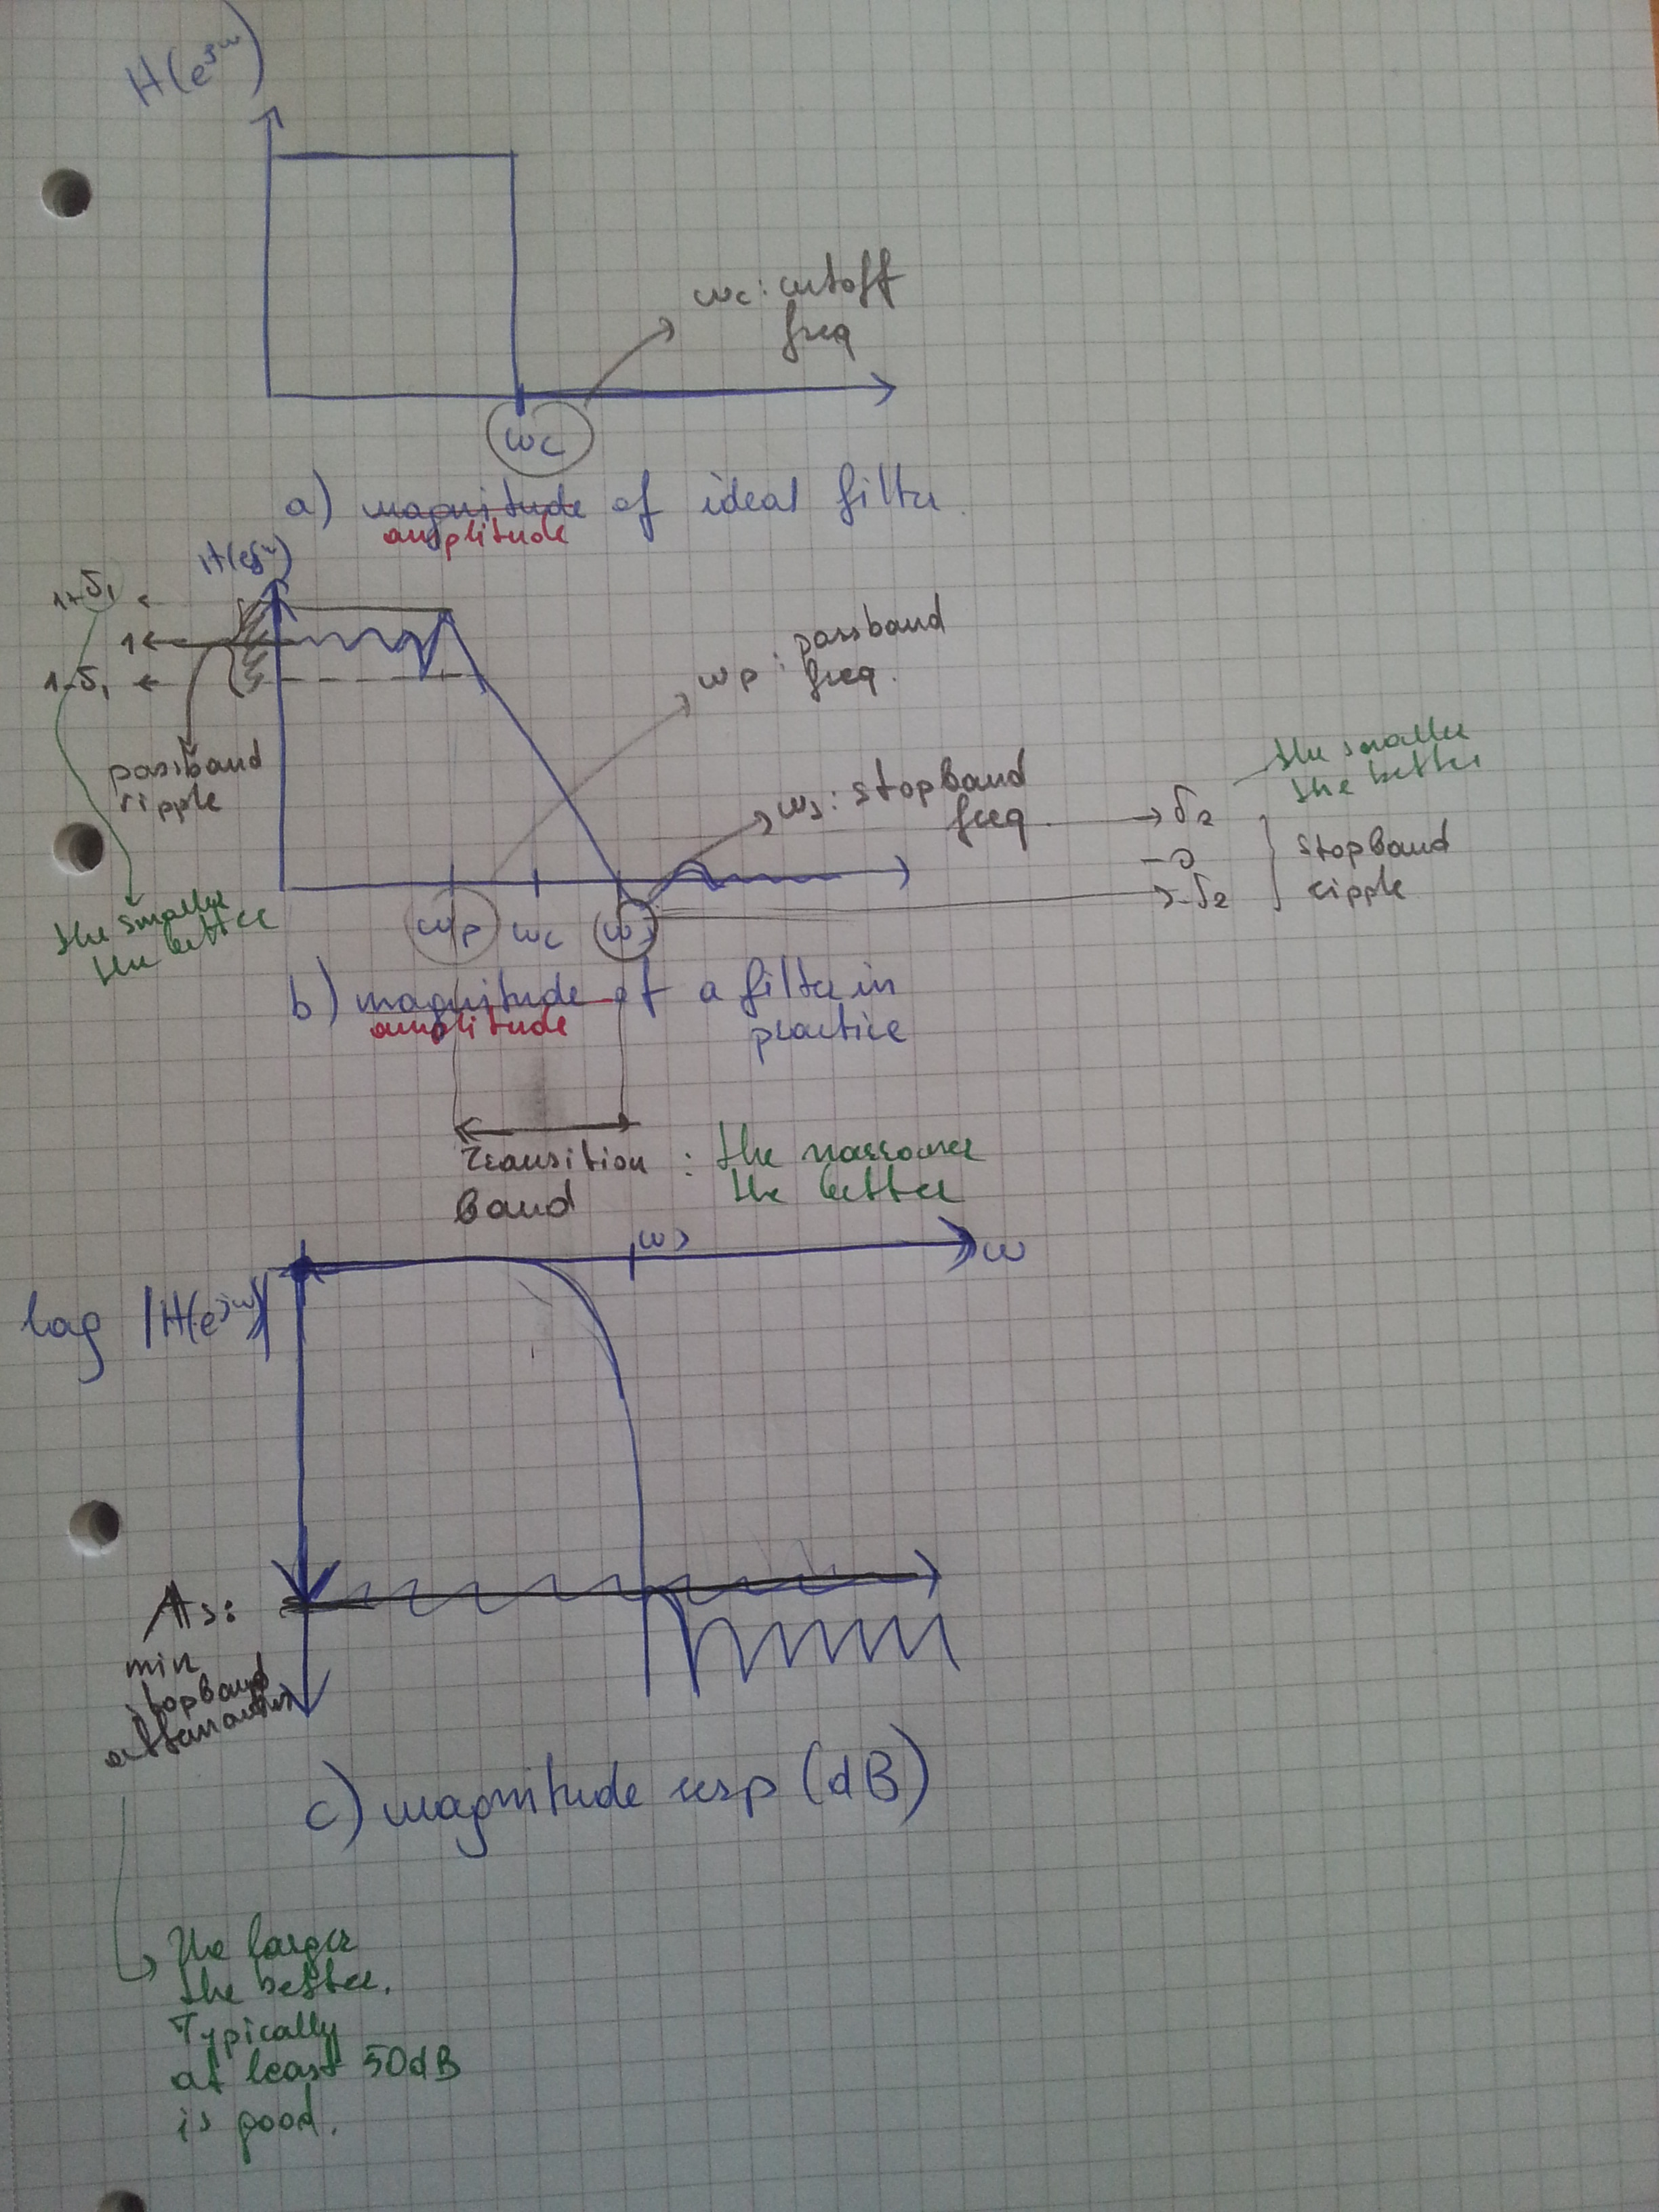
\includegraphics[scale=0.20]{fig/fir_design.jpg}
\label{fig:design}
\caption{FIR filter design specs}
\end{figure}


% https://www.youtube.com/watch?v=VXwXkME9uWU&list=PLMn2aW3wpAtOqo0g0OnHndXB1LnYBeMaX&index=1
\end{document}


